\documentclass[10pt,twocolumn]{article}

% ---------- Packages ----------
\usepackage[utf8]{inputenc}
\usepackage[T1]{fontenc}
\usepackage[margin=0.70in]{geometry}
\usepackage{amsmath,amssymb}
\usepackage{graphicx}
\usepackage{booktabs}
\usepackage{caption}
\usepackage{subcaption}
\usepackage{cite}
\usepackage[expansion=false]{microtype}
\usepackage{url}
\usepackage{xcolor}
\usepackage[hidelinks]{hyperref}

\captionsetup{font=small,labelfont=bf}
\captionsetup[sub]{font=footnotesize}
\graphicspath{{figures/}}

\setlength{\parskip}{0.08em}

% ---------- Float packing (fit within 7 pages) ----------
\renewcommand{\topfraction}{0.94}
\renewcommand{\bottomfraction}{0.75}
\renewcommand{\textfraction}{0.05}
\renewcommand{\floatpagefraction}{0.72}
\renewcommand{\dbltopfraction}{0.94}
\renewcommand{\dblfloatpagefraction}{0.72}
\setcounter{topnumber}{4}
\setcounter{bottomnumber}{3}
\setcounter{totalnumber}{6}
\setcounter{dbltopnumber}{4}

\setlength{\textfloatsep}{5pt plus 1pt minus 1pt}
\setlength{\floatsep}{5pt plus 1pt minus 1pt}
\setlength{\dbltextfloatsep}{5pt plus 1pt minus 1pt}
\setlength{\dblfloatsep}{5pt plus 1pt minus 1pt}
\setlength{\intextsep}{5pt plus 1pt minus 1pt}
\setlength{\abovecaptionskip}{4pt}
\setlength{\belowcaptionskip}{2pt}

% ---------- Title ----------
\title{\vspace{-1.8em}\textbf{Adaptive Operator Selection for the Travelling\\
Salesman Problem via Tabular Q-Learning}\vspace{-0.3em}}
\author{\"Ozlem Akyaz \qquad S{\i}la Erda\u{g}\\[0.2em]
\small Reinforcement Learning Applications for Combinatorial Optimization\\
\small AIE635 Reinforcement Learning Final Project }
\date{}

\begin{document}

\twocolumn[
\begin{@twocolumnfalse}
\maketitle
\vspace{-2.2em}
\begin{abstract}
\noindent
This paper examines whether a state-aware, learned selection rule can
distribute local-search operators across an optimization run more profitably
than relying on any single operator for the symmetric travelling salesman
problem (TSP). The iterated-local-search loop is modelled as a Markov decision
process in which the state captures solution quality, whether the previous move
was improving, the elapsed fraction of the budget, and which operator was last
used; a tabular Q-learning agent is then trained to pick among
best-improvement 2-opt, swap, relocate, and random restart. Experiments span
four TSPLIB instances with 30 seeded repetitions each, and the learned selector
reaches mean gaps to the optimum of 3.90\% (eil51), 0.51\% (berlin52), and
3.34\% (st70), beating the single strongest operator with statistical
significance on all three (paired Wilcoxon, $p<0.05$). For the largest
benchmark (kroA100), however, a dedicated fixed 2-opt achieves a lower gap
(5.21\% against 6.23\%, $p=0.031$), demonstrating that the advantage of
adaptive selection narrows---and ultimately reverses---as the instance grows.
Two alternative reward definitions are found to yield identical behaviour; a
stagnation-responsive exploration schedule is shown to produce the tightest gaps
together with the lowest restart frequency. A further investigation reveals
that the adaptive schedule is acutely sensitive to the signal feeding its
stagnation detector: replacing incumbent improvement with global-best
improvement causes exploration to saturate and degrades the policy to a level
below every baseline---this pitfall is characterized and discussed. An
important caveat accompanies all findings: the state encoding bins solution
quality using the known optimal tour length, an oracle quantity unavailable in
practice; when a Q-table trained on the smaller instances is transferred to the
larger ones under identical hyper-parameters, performance is observed to be
statistically indistinguishable from training from scratch. Lastly, a seemingly
meaningful operator pairing---a swap followed by 2-opt with conditional
probability 1.0---is demonstrated to be a statistical artefact arising from
2-opt's overwhelming share of all improving moves rather than a genuine
learned strategy.
\vspace{0.4em}
\end{abstract}
\end{@twocolumnfalse}
]

% ============================================================
\section{Introduction}
% ============================================================
Given a set of cities, the travelling salesman problem (TSP) seeks the
shortest Hamiltonian cycle and stands as one of the most studied NP-hard
combinatorial optimization problems. Iterative improvement via neighbourhood
operators---2-opt edge exchange, city swap, and city relocation---remains a
practical backbone, and leading inexact solvers such as the Lin--Kernighan
heuristic and its Helsgaun variant are founded on precisely such
moves~\cite{lin1973,helsgaun2000}. A well-known empirical pattern, however, is
that no single operator is uniformly best across an entire search trajectory:
aggressive neighbourhood restructuring tends to yield rapid early progress,
while diversification mechanisms become valuable once refinement stalls. This
pattern provides the rationale for adaptive operator selection, where the choice
of which move to apply next is conditioned on the current search
state~\cite{burke2013,meignan2010}.

The present study asks whether tabular Q-learning~\cite{watkins1992,sutton2018}
is capable of acquiring such a conditional selection policy for the TSP. Three
contributions are offered: (i)~a compact MDP formulation of iterated local
search that encodes the search state into 120 discrete values and provides four
operators as actions (Section~\ref{sec:method}); (ii)~a systematic experimental
evaluation on four TSPLIB instances, each repeated 30 times under paired seeds,
comparing the trained policy against every individual fixed operator and a
uniform-random selector (Section~\ref{sec:results}); and (iii)~an examination of
reward shaping alternatives, exploration schedules and their sensitivity to the
signal feeding the stagnation counter, operator-transition patterns, and
cross-instance transfer.

\paragraph{An upfront caveat.} Solution quality is discretized by computing the
relative gap to the \emph{known} optimal tour length. Because this optimum is
unavailable in any real deployment, this constitutes an oracle feature that
artificially enriches the agent's awareness. It is retained because the primary
interest lies in the operator-selection mechanism itself, but it represents the
single largest threat to external validity and is revisited in
Sections~\ref{sec:transfer} and~\ref{sec:discussion}.

% ============================================================
\section{Related Work}
% ============================================================
The origins of local-search improvement for the TSP trace back to the 2-opt
exchange introduced by Croes~\cite{croes1958} and the variable-depth procedure
of Lin and Kernighan~\cite{lin1973}; Helsgaun's refinement of the latter (LKH)
continues to rank among the best-performing inexact algorithms for
large-scale instances~\cite{helsgaun2000}. Iterated local
search~\cite{lourenco2003} wraps such moves inside a perturbation--restart
framework, bearing a close structural resemblance to the episodic procedure
controlled in the present work. The broader problem of choosing operators
on-the-fly falls within the hyper-heuristics
field~\cite{burke2013}. Reinforcement learning fits naturally because operator
selection is inherently sequential. Meignan et al.\ employ reinforcement
learning to manage the ordering of neighbourhood operators inside a
coalition-based metaheuristic for vehicle-routing
problems~\cite{meignan2010}. In a more recent line of research, da Costa
et al.\ apply deep reinforcement learning to directly learn a 2-opt move
proposal policy and achieve competitive optimality gaps on TSPLIB-scale
instances~\cite{dacosta2020}. The current work opts for a deliberately simpler
setup---tabular Q-learning atop a manually designed state space---so that the
resulting policy remains fully transparent and the impact of each design
decision can be cleanly attributed. Exploration is handled through
$\varepsilon$-greedy variants, one of which adapts its rate based on
search progress, drawing on the value-difference-based exploration
concept~\cite{tokic2010}.

% ============================================================
\section{Methodology}\label{sec:method}
% ============================================================
\subsection{Modelling the search as a Markov decision process}
A single optimization run constitutes one episode lasting $T$ steps. On every
step the agent reads a discretized state~$s$, picks an operator~$a$, applies it
to the current tour, and collects a scalar reward. The state is the product of
four factors:
\[
s = \bigl(q,\; m,\; \sigma,\; o_{-1}\bigr),
\]
defined as follows:
\begin{itemize}\itemsep0.1em
  \item quality band $q\in\{0,\dots,4\}$: the incumbent's relative gap to the
        optimum, bucketed at thresholds of $5\%$, $15\%$, $30\%$, and $50\%$;
  \item improvement indicator $m\in\{0,1\}$: set to one when the most recent
        move reduced the tour length;
  \item budget phase $\sigma\in\{0,1,2\}$: the first, second, and final third
        of the iteration budget;
  \item preceding operator $o_{-1}\in\{0,1,2,3\}$.
\end{itemize}
Multiplying the factor cardinalities gives $5\times2\times3\times4 = 120$
distinct states. As highlighted earlier, $q$ relies on the optimal tour length
and therefore constitutes oracle knowledge.

\subsection{Available operators (actions)}
Four operators with a shared interface form the action set:
\begin{enumerate}\itemsep0.1em
  \item \textbf{2-opt (best improvement):} a sample of up to $\min(2n,100)$
        edge pairs is evaluated using the four-edge delta formula, and the
        reversal yielding the largest cost reduction is executed;
  \item \textbf{swap:} two cities selected uniformly at random exchange their
        positions in the tour;
  \item \textbf{relocate:} a randomly chosen city is extracted and reinserted
        at a different location;
  \item \textbf{restart:} the entire incumbent is discarded and replaced with
        a fresh random permutation.
\end{enumerate}
For the three non-restart operators, a worsening move is still accepted with
probability $0.01$, providing a mild simulated-annealing-like perturbation;
restart unconditionally replaces the incumbent.

\subsection{Reward definitions}
Two reward signals are contrasted. The first, $R_1$, equals the raw change in
tour length,
$R_1=\ell_{\mathrm{prev}}-\ell_{\mathrm{new}}$, and is applied identically to
all four operators (a restart therefore receives a large negative value
proportional to the disruption it causes).
The second, $R_2$, augments $R_1$ with a fixed bonus of $100$ each time the
move establishes a new global best:
\[
R_2 = (\ell_{\mathrm{prev}}-\ell_{\mathrm{new}})
      + 100\cdot\mathbf{1}\!\left[\ell_{\mathrm{new}}<\ell^{*}_{\mathrm{global}}\right].
\]

\subsection{Learning procedure and exploration control}
The agent employs tabular Q-learning~\cite{watkins1992} with a step size of
$\alpha=0.1$ and a discount factor of $\gamma=0.9$, applying the standard
Bellman update
$Q(s,a)\leftarrow Q(s,a)+\alpha\bigl[r+\gamma\max_{a'}Q(s',a')-Q(s,a)\bigr]$.
Three $\varepsilon$-greedy schedules are tested: a fixed rate of
$\varepsilon=0.1$; an exponentially decaying rate starting at $1.0$, flooring
at $0.01$, with a per-step factor of $0.998$; and an adaptive scheme that
decreases $\varepsilon$ whenever the incumbent improves and increases it by
$0.05$ once $50$ consecutive non-improving steps have elapsed, following the
spirit of value-difference-based exploration~\cite{tokic2010}. Crucially, the
event that resets the stagnation counter in the adaptive variant is taken to be
improvement of the \emph{incumbent} solution---the identical event that
determines the sign of the reward and the improvement flag $m$. The
ramifications of choosing a different signal are examined in
Section~\ref{sec:signal}.

\subsection{Experimental protocol}
Four symmetric TSPLIB benchmarks~\cite{reinelt1991} are employed: eil51,
berlin52, st70, and kroA100, whose known optimal tour lengths are $426$,
$7542$, $675$, and $21{,}282$ respectively. Inter-city distances adhere to the
TSPLIB \texttt{EUC\_2D} convention, in which the Euclidean distance is rounded
to the nearest integer via $\lfloor d+0.5\rfloor$. Unless noted otherwise, each
configuration runs for $T=3000$ steps and is repeated across $30$ independent
random seeds; the same seed sequence is shared among all compared strategies,
enabling paired statistical testing with the Wilcoxon signed-rank test. Results
are summarized by the percentage optimality gap
$\mathrm{gap}=100(\ell-\ell^{*})/\ell^{*}$, expressed as
mean\,$\pm$\,standard deviation. The two smaller instances (eil51 and berlin52)
serve as training data for the transfer experiment; st70 and kroA100 are
reserved for testing.

% ============================================================
\section{Results}\label{sec:results}
% ============================================================
\subsection{Primary performance comparison}
Table~\ref{tab:main} presents the optimality gaps achieved by the trained
policy alongside those of the four individual fixed operators and the
uniform-random selector. On three of the four benchmarks---eil51, berlin52, and
st70---the Q-learning agent produces the lowest mean gap. Relative to fixed
2-opt, which is far and away the most effective single operator, the
improvement reaches statistical significance on all three of these instances
(paired Wilcoxon: $p=0.0028$, $p=3.8\times10^{-6}$, $p=0.021$;
Table~\ref{tab:wilcoxon}). Comparisons with the swap, relocate, and
restart-only strategies yield overwhelming margins everywhere ($p<10^{-5}$).

The pattern breaks on the largest benchmark, kroA100: here, fixed 2-opt
finishes at $5.21\%$ while the learned selector reaches only $6.23\%$, a
statistically significant shortfall ($p=0.031$). Rather than masking this
reversal through aggregation, it is reported directly: the payoff from learned
selection is not universal and appears to weaken as instances grow larger. One
plausible interpretation, reinforced by the operator-usage statistics below and
the transfer analysis in Section~\ref{sec:transfer}, is that on larger search
spaces 2-opt alone already harvests the bulk of the achievable improvement,
leaving minimal scope for a switching policy to contribute additional value;
simultaneously, the oracle quality feature provides progressively less useful
guidance as the distribution of attainable gaps shifts.

A closer look at the random-selector comparison reveals subtleties that a
headline average would obscure. On the two smaller training instances the
learned policy does not significantly outperform random operator selection
($p=0.52$ on eil51, $p=0.067$ on berlin52); the advantage emerges clearly only
on the larger unseen instances ($p=0.0066$ on st70, $p=6.9\times10^{-7}$ on
kroA100). The random strategy collapses on kroA100 ($14.16\%$) because three
out of its four operators are ineffective there, whereas the trained agent
directs nearly all effort toward 2-opt. Convergence trajectories appear in
Fig.~\ref{fig:conv}.

\subsection{Operator-transition patterns and the ``synergy'' artefact}
An obvious question is whether the trained policy learns a productive ordering
of operators. To investigate, a transition matrix $C_{ij}$ was accumulated
across all 30 runs, recording how frequently an improving move by operator~$i$
is followed by the next improving move using operator~$j$ (restarts are
excluded from this count). Fig.~\ref{fig:trans} displays the matrices for eil51
and kroA100. The row-normalized conditional
$P(\text{next}=\text{2-opt}\mid\text{prev}=\text{swap})$ equals $1.00$ on both
instances, an observation that could be read as a learned ``swap-followed-by-2-opt''
combination akin to a variable-depth search move. This reading is misleading.
The unconditional marginal $P(\text{next}=\text{2-opt})$ already stands at
$0.997$ (eil51) and $0.998$ (kroA100): 2-opt is responsible for more than
$99.7\%$ of all improving moves ($42{,}497$ on eil51, compared with just $70$
for swap and $77$ for relocate). Since virtually every improving step is a
2-opt step, every operator---including swap---is followed by 2-opt at
approximately the base rate, and the swap row's tiny denominator ($70$
transitions) trivially normalizes to $1.00$. The conditional therefore conveys
no information beyond what the marginal already supplies. The conclusion is
that the policy's benefit stems from channelling effort toward 2-opt and using
the weaker operators and restart only for occasional diversification, not from
any intentionally orchestrated operator sequence. The learned Q-values
(Fig.~\ref{fig:qtable}) corroborate this picture: 2-opt holds the highest
action-value across most quality bands.

\subsection{Effect of reward shaping}
Across both training instances the two reward signals produced gap
distributions that are identical run-for-run over all 30 paired seeds (maximum
pointwise difference of $0.0$; restart counts match exactly at $37.0$ on eil51
and $35.6$ on berlin52). Under a common seed the global-best bonus in $R_2$
shifts the Q-table entries but never alters the greedily selected operator
within the given budget, so both agents trace out the same trajectory. These
results provide no support for the hypothesis that the global-best bonus
improves learning; the more parsimonious $R_1$ is therefore preferred.
Convergence plots appear in Fig.~\ref{fig:reward}. (The run-level identity is
an artefact of these specific seeds and this budget length; under a longer
horizon or different seeds only statistical equivalence, not exact coincidence,
would be anticipated.)

\subsection{Comparison of exploration schedules}
Table~\ref{tab:explore} summarizes the three $\varepsilon$-greedy variants. The
adaptive stagnation-aware schedule delivers the tightest gaps on both training
instances ($3.90\%$ on eil51, $0.51\%$ on berlin52) while simultaneously
incurring the fewest restarts ($37.0$ and $35.6$), in contrast to
$77.1$/$76.1$ for constant $\varepsilon$ and $126.4$/$126.6$ for the
exponential decay scheme. Exponential decay begins with near-random action
selection, which leads to considerable early thrashing and inflated restart
counts without a proportionate quality gain. The constant and decaying
schedules perform similarly to each other and are both clearly inferior to the
adaptive alternative. Fig.~\ref{fig:eps} visualizes the convergence curves and
the $\varepsilon$ trajectory over time.

\subsection{Dependence on the exploration-signal
choice}\label{sec:signal}
The positive results of the adaptive schedule turn out to hinge on
\emph{which} notion of improvement drives the stagnation counter. A controlled
comparison was conducted under otherwise identical settings (raw-improvement
reward, adaptive schedule, 30 runs): in one arm the counter is reset whenever
the \emph{incumbent} tour improves (the convention used throughout this work);
in the other it is reset only when a new \emph{global best} is established.
Table~\ref{tab:signal} summarizes the outcome.

Under the global-best signal, $\varepsilon$ rises steadily toward its upper
bound as soon as the global record stagnates---an event that typically occurs
early, once 2-opt's initial descent settles into a local optimum---and then
stays at that ceiling for the remainder of the episode. The resulting
near-uniform exploration causes restart to be invoked approximately $500$ times
per episode, roughly $14$ times more often than under the incumbent signal. The
mean gap climbs to $9.67\%$ (eil51) and $7.54\%$ (berlin52), exceeding the
gaps of fixed 2-opt and even of the random selector reported in
Table~\ref{tab:main}. The practical takeaway is that a stagnation-triggered
exploration mechanism must be linked to a signal that continues to fire during
productive search. If it is instead linked to a quantity that inevitably
plateaus (such as the global best), the mechanism's own $\varepsilon$ ceiling
effectively transforms the policy into a near-random selector, silently
eliminating the advantage of learned operator selection. A related failure mode
was observed when restart was assigned a small constant penalty rather than the
disruption-scaled reward $R_1$; the fixed cost fails to capture the true
expense of discarding the incumbent and, under temporal discounting, leaves
restart appealing. Both observations reinforce the importance of keeping the
reward and exploration signals aligned with the event they are intended to
reflect.

\subsection{Transfer to held-out instances}\label{sec:transfer}
A single Q-table was trained on the two small instances (eil51 and berlin52),
after which two agents were compared on each held-out instance under matching
hyper-parameters ($\alpha=0.1$, adaptive~$\varepsilon$): one seeded with the
transferred table (warm-start) and one beginning from a blank table. This
paired design was chosen deliberately---an alternative that combined the
pre-trained table with a smaller learning rate and a low fixed $\varepsilon$
would confound the effect of transfer with that of a weaker learner.

With the hyper-parameters equalized, transfer has no discernible effect: on
st70 the warm-started agent reaches $2.99\%$ versus $3.34\%$ for the
from-scratch agent ($p=0.41$), and on kroA100 the figures are $6.32\%$ versus
$6.23\%$ ($p=0.65$); neither gap is statistically significant
(Fig.~\ref{fig:gen}). Transfer is therefore essentially neutral in this
setting. The explanation lies in the oracle quality feature: because the band
index $q$ is defined relative to each instance's own optimum, the state
distribution encountered during search shifts between instances, and Q-values
calibrated on one do not carry meaningful information to another. This outcome
is interpreted as a limitation of the chosen state design rather than as
evidence for or against transfer learning in general.

\subsection{Illustrative best tours}
Fig.~\ref{fig:tour} displays the shortest tours discovered by the learned
policy on the smallest and largest instances, achieving optimality gaps of
$1.88\%$ and $1.48\%$ respectively.

% ============================================================
\section{Discussion and Limitations}\label{sec:discussion}
% ============================================================
The headline result is modest rather than dramatic. A learned, state-conditioned
operator-selection rule can beat any single fixed operator as well as a
uniform-random selector, yet the improvement depends strongly on the instance:
it is most pronounced on small and medium benchmarks and vanishes---turning
into a deficit against a well-tuned 2-opt---on the largest instance
investigated. Several factors circumscribe these conclusions.

The most consequential limitation is the \texttt{quality\_band} feature's
dependence on the true optimal tour length. This oracle information would not
be available in any practical application and almost certainly flatters the
agent's ability to discriminate among states; a realistic alternative would
require a surrogate such as the ratio to the best tour encountered so far or to
a lower bound. The neutral transfer outcome reported in
Section~\ref{sec:transfer} is a direct manifestation of this dependency.

Additionally, the operator portfolio is heavily skewed toward 2-opt, which
accounts for over $99.7\%$ of all improving moves. The remaining perturbation
operators make negligible independent contributions, which simultaneously
explains why fixed 2-opt is such a formidable baseline and constrains the margin
available to any learned selector. Testing with a more balanced set of
individually competitive operators (for example, Or-opt, 3-opt, or
segment-insertion moves) would provide a fairer evaluation of the adaptive
selection concept.

As shown in Section~\ref{sec:signal}, the adaptive exploration schedule is
fragile with respect to the signal feeding its stagnation detector; the
favourable outcomes presented here depend on coupling that detector to incumbent
improvement. This sensitivity constitutes a finding in its own right---adaptive
exploration heuristics can fail catastrophically and without obvious warning
when the triggering signal becomes uninformative---and it highlights the
necessity of reporting such design choices transparently.

Lastly, the experimental scope is restricted to four Euclidean instances of at
most $100$ cities under a single family of paired seeds; the reversal observed
on kroA100 should be replicated across additional and larger instances before
broad generalizations are attempted. The state discretization, too, is manually
crafted; learning the representation, or substituting a function approximator
for the table as in~\cite{dacosta2020}, is a natural avenue for future work.

% ============================================================
\section{Conclusion}
% ============================================================
An iterated-local-search procedure for the TSP was framed as a Markov decision
process and a tabular Q-learning agent was trained to select among 2-opt, swap,
relocate, and restart operators. Across 30 runs per configuration the trained
policy achieved significantly lower optimality gaps than the best fixed operator
on three out of four TSPLIB instances, while a dedicated fixed 2-opt proved
superior on the largest instance, indicating that the returns from adaptive
selection diminish as the problem scales. The two reward variants tested were
statistically indistinguishable, and an adaptive stagnation-aware exploration
schedule produced the best gaps alongside the lowest restart counts---contingent
on the stagnation counter being driven by incumbent improvement; substituting
global-best improvement was demonstrated to saturate exploration and push the
policy below every baseline. No true operator synergy was uncovered: the
ostensible swap-to-2-opt pairing is a statistical artefact of 2-opt's
overwhelming dominance among improving moves. Owing to the oracle quality
feature embedded in the state encoding, cross-instance transfer proved neutral
when hyper-parameters were controlled. Eliminating the oracle dependency and
diversifying the operator portfolio are regarded as the most pressing
directions for rendering learned operator selection genuinely practical on the
TSP.

% ============================================================
% Figures and Tables
% ============================================================

\begin{table*}[t]
\centering
\caption{Mean optimality gap (\%) $\pm$ standard deviation across 30 runs.
The lowest gap per instance is shown in \textbf{bold}. Training instances:
eil51, berlin52.}
\label{tab:main}
\small
\begin{tabular}{lcccccc}
\toprule
Instance & Q-Learning & Fixed 2-opt & Fixed swap & Fixed relocate & Fixed restart & Random \\
\midrule
eil51    & \textbf{3.90$\pm$1.00} & 5.32$\pm$2.00 & 23.30$\pm$5.20 & 21.36$\pm$4.74 & 23.99$\pm$5.47 & 4.22$\pm$1.60 \\
berlin52 & \textbf{0.51$\pm$1.26} & 4.56$\pm$2.39 & 17.72$\pm$3.67 & 17.40$\pm$3.60 & 18.04$\pm$3.67 & 1.65$\pm$2.16 \\
st70     & \textbf{3.34$\pm$1.41} & 4.59$\pm$2.51 & 26.32$\pm$4.56 & 24.65$\pm$5.31 & 27.06$\pm$4.28 & 5.11$\pm$2.36 \\
kroA100  & 6.23$\pm$1.98 & \textbf{5.21$\pm$2.22} & 27.28$\pm$3.44 & 27.15$\pm$3.76 & 27.67$\pm$3.70 & 14.16$\pm$6.91 \\
\bottomrule
\end{tabular}
\end{table*}

\begin{figure*}[t]
\centering
\begin{subfigure}{0.245\textwidth}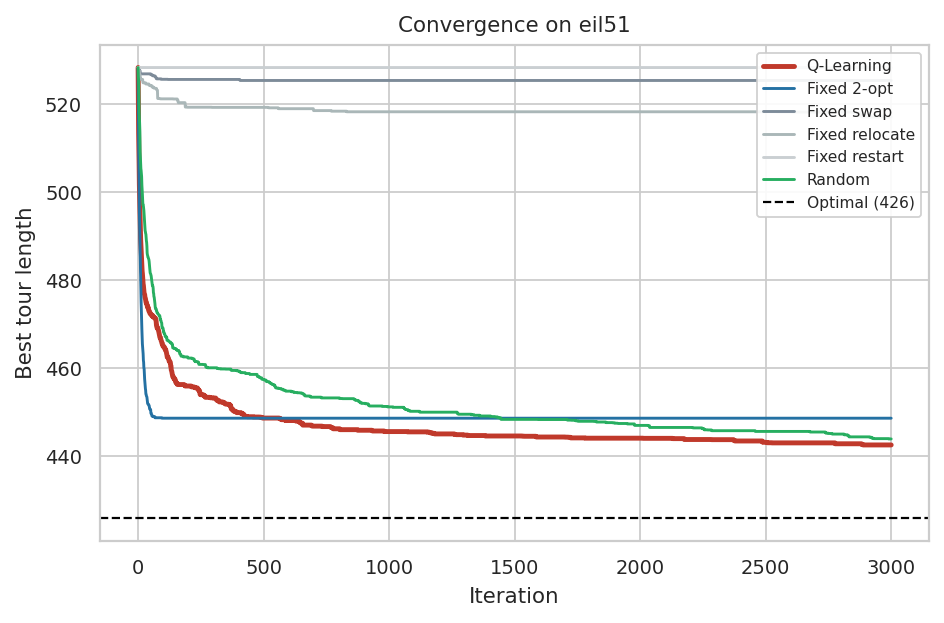
\includegraphics[width=\linewidth]{convergence_eil51.png}\caption{eil51}\end{subfigure}\hfill
\begin{subfigure}{0.245\textwidth}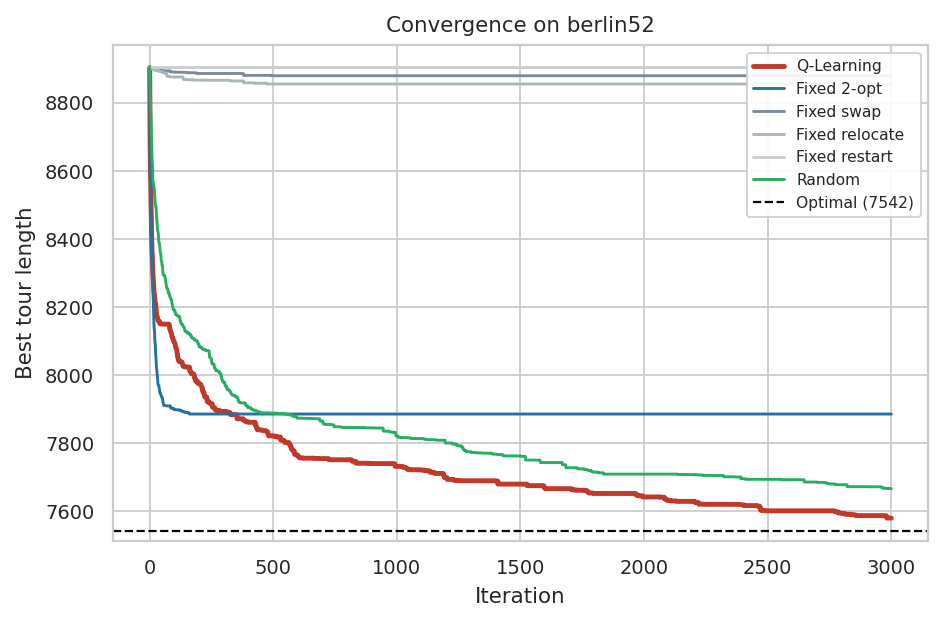
\includegraphics[width=\linewidth]{convergence_berlin52.png}\caption{berlin52}\end{subfigure}\hfill
\begin{subfigure}{0.245\textwidth}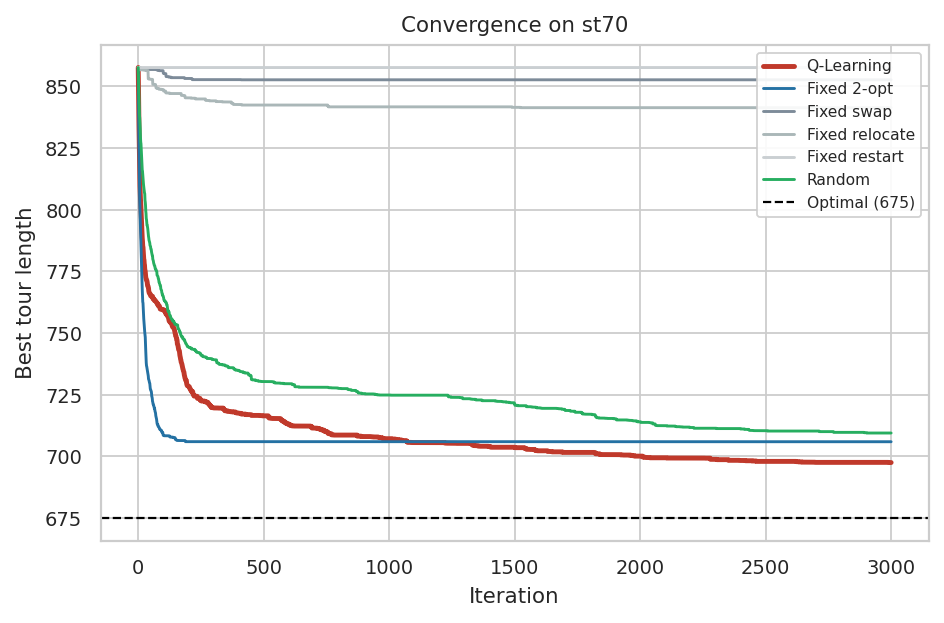
\includegraphics[width=\linewidth]{convergence_st70.png}\caption{st70}\end{subfigure}\hfill
\begin{subfigure}{0.245\textwidth}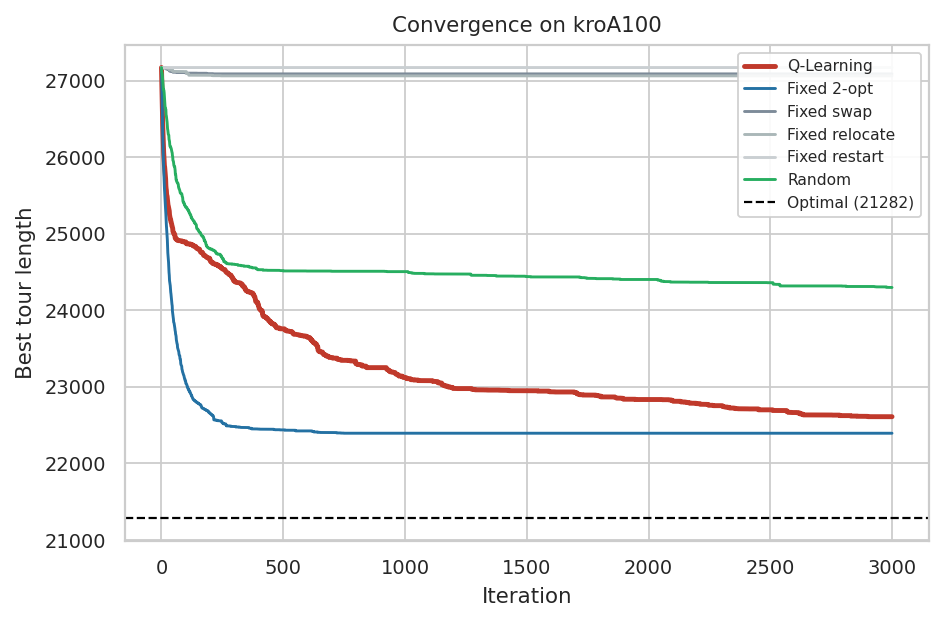
\includegraphics[width=\linewidth]{convergence_kroA100.png}\caption{kroA100}\end{subfigure}
\caption{Best-so-far tour length, averaged over 30 runs. The trained policy
matches or surpasses fixed 2-opt on eil51, berlin52, and st70; on kroA100 fixed
2-opt holds a slight edge.}
\label{fig:conv}
\end{figure*}

\begin{table}[t]
\centering
\caption{Paired Wilcoxon signed-rank test comparing the trained policy to the
two strongest baselines. $\Delta$ denotes the mean gap difference (Q-learning
$-$ baseline); a negative value favours the trained policy. ``n.s.'' indicates
non-significance at $\alpha=0.05$.}
\label{tab:wilcoxon}
\small
\begin{tabular}{lcccc}
\toprule
 & \multicolumn{2}{c}{vs.\ Fixed 2-opt} & \multicolumn{2}{c}{vs.\ Random} \\
\cmidrule(lr){2-3}\cmidrule(lr){4-5}
Instance & $\Delta$ & $p$ & $\Delta$ & $p$ \\
\midrule
eil51    & $-1.42$ & $0.0028$ & $-0.32$ & $0.52$ (n.s.) \\
berlin52 & $-4.05$ & $3.8\mathrm{e}{-6}$ & $-1.15$ & $0.067$ (n.s.) \\
st70     & $-1.25$ & $0.021$ & $-1.77$ & $0.0066$ \\
kroA100  & $+1.02$ & $0.031$ & $-7.93$ & $6.9\mathrm{e}{-7}$ \\
\bottomrule
\end{tabular}
\end{table}

\begin{table}[t]
\centering
\caption{Exploration schedules: mean gap (\%) and average restart count per
episode across 30 runs.}
\label{tab:explore}
\small
\begin{tabular}{llcc}
\toprule
Instance & Schedule & Gap (\%) & Restarts \\
\midrule
          & Constant $\varepsilon{=}0.1$  & 4.54$\pm$1.20 & 77.1 \\
eil51     & Exponential decay             & 4.44$\pm$1.56 & 126.4 \\
          & Adaptive (stagnation)         & \textbf{3.90$\pm$1.00} & \textbf{37.0} \\
\midrule
          & Constant $\varepsilon{=}0.1$  & 1.62$\pm$2.27 & 76.1 \\
berlin52  & Exponential decay             & 1.73$\pm$2.45 & 126.6 \\
          & Adaptive (stagnation)         & \textbf{0.51$\pm$1.26} & \textbf{35.6} \\
\bottomrule
\end{tabular}
\end{table}

\begin{table}[t]
\centering
\caption{Impact of the signal feeding the adaptive schedule's stagnation
counter (raw-improvement reward, 30 runs). When the counter tracks the global
best, exploration saturates and restarts increase approximately $14$-fold,
pushing the policy below every baseline listed in Table~\ref{tab:main}.}
\label{tab:signal}
\small
\begin{tabular}{lcccc}
\toprule
 & \multicolumn{2}{c}{Incumbent signal} & \multicolumn{2}{c}{Global-best signal} \\
\cmidrule(lr){2-3}\cmidrule(lr){4-5}
Instance & Gap (\%) & Restarts & Gap (\%) & Restarts \\
\midrule
eil51    & \textbf{3.90$\pm$1.00} & \textbf{37.0} & 9.67$\pm$6.38 & 527.2 \\
berlin52 & \textbf{0.51$\pm$1.26} & \textbf{35.6} & 7.54$\pm$3.80 & 535.9 \\
\bottomrule
\end{tabular}
\end{table}

\begin{figure*}[t]
\centering
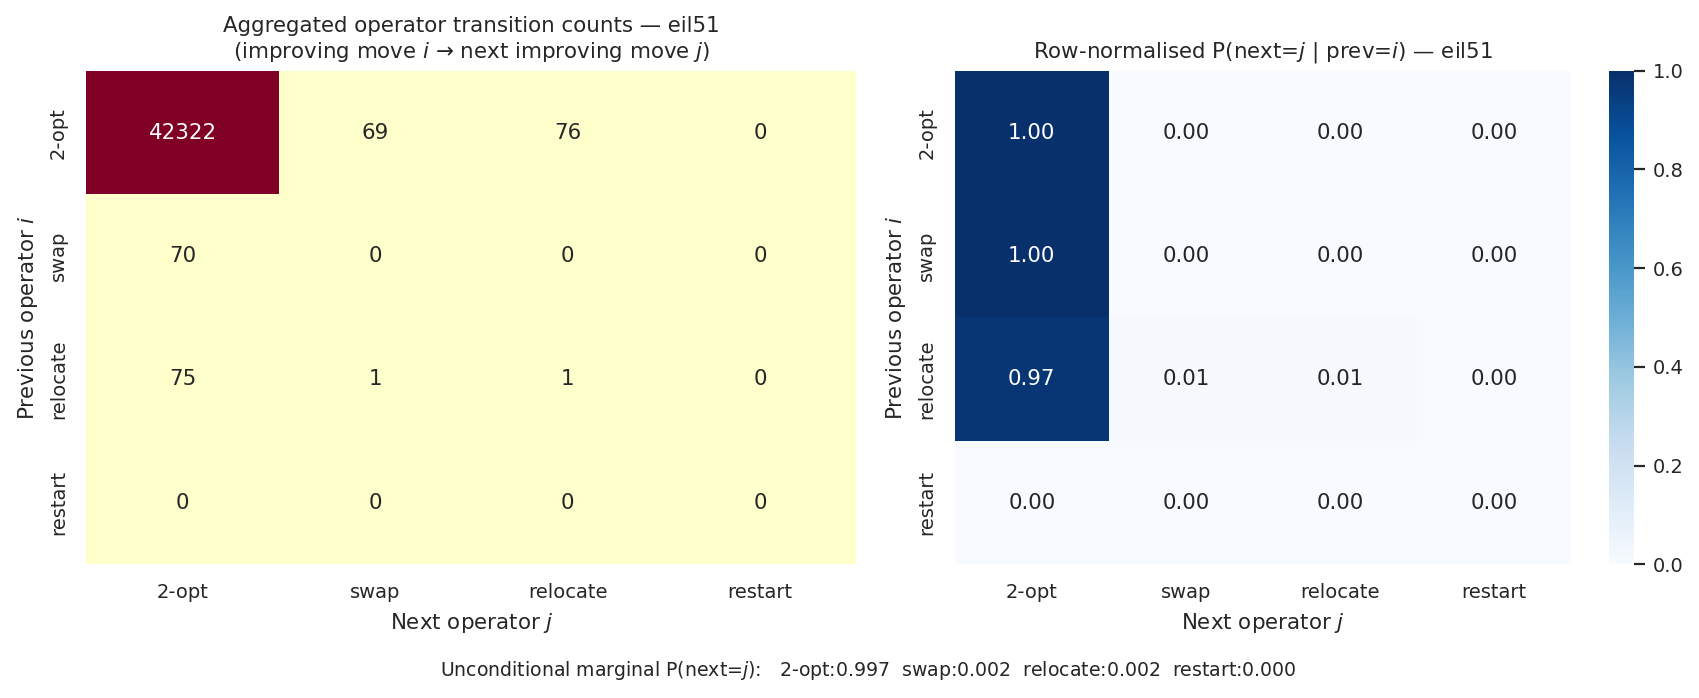
\includegraphics[width=0.58\textwidth]{transition_eil51.png}\\[0.2em]
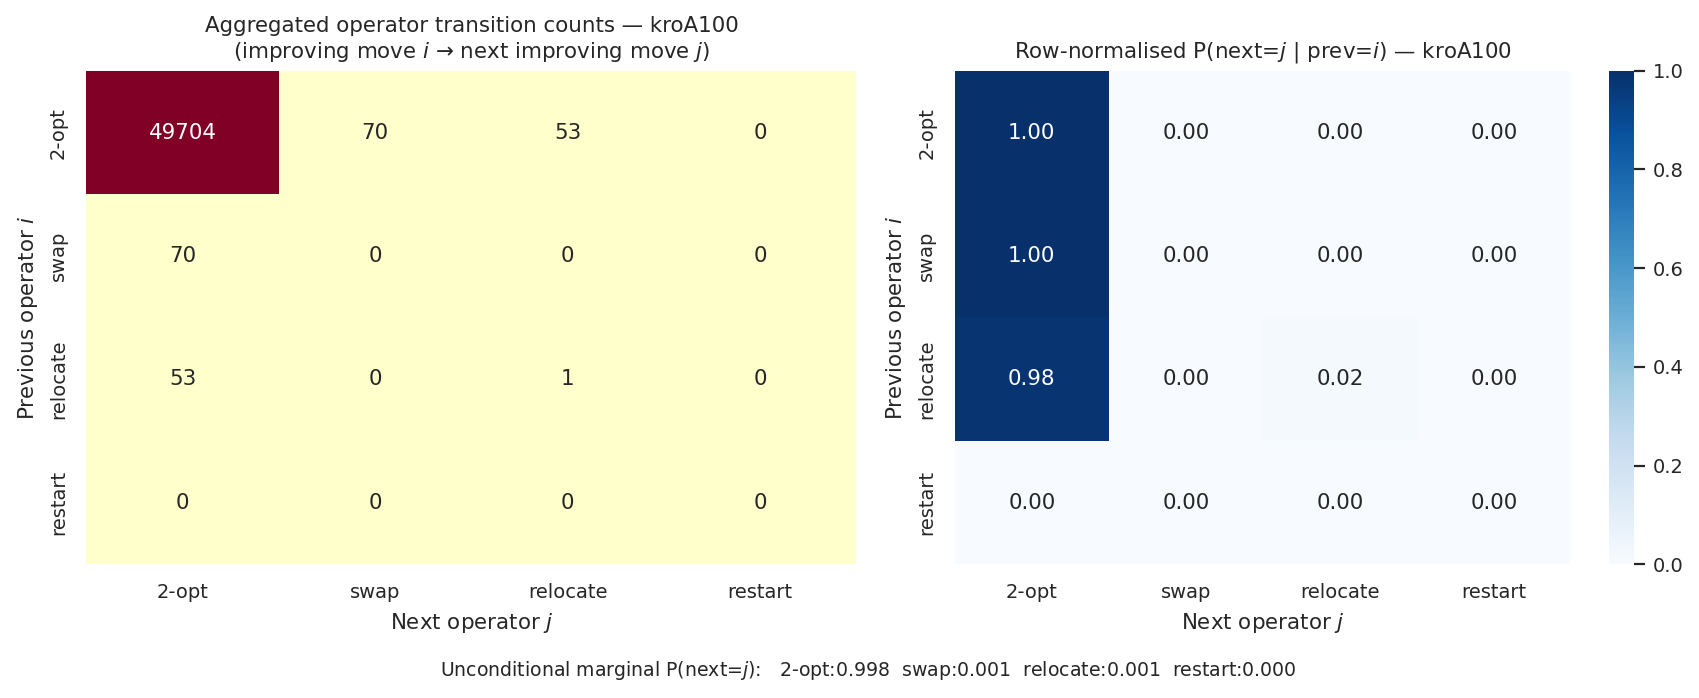
\includegraphics[width=0.58\textwidth]{transition_kroA100.png}
\caption{Cumulative operator-transition counts (left panels) and
row-normalized transition probabilities (right panels) for eil51 (upper row) and
kroA100 (lower row). The near-unity conditional
$P(\text{next}=\text{2-opt}\mid\cdot)\approx1$ simply mirrors the unconditional
marginal shown below each panel and does not signal a deliberate operator
pairing.}
\label{fig:trans}
\end{figure*}

\begin{figure}[t]
\centering
\begin{subfigure}{0.49\linewidth}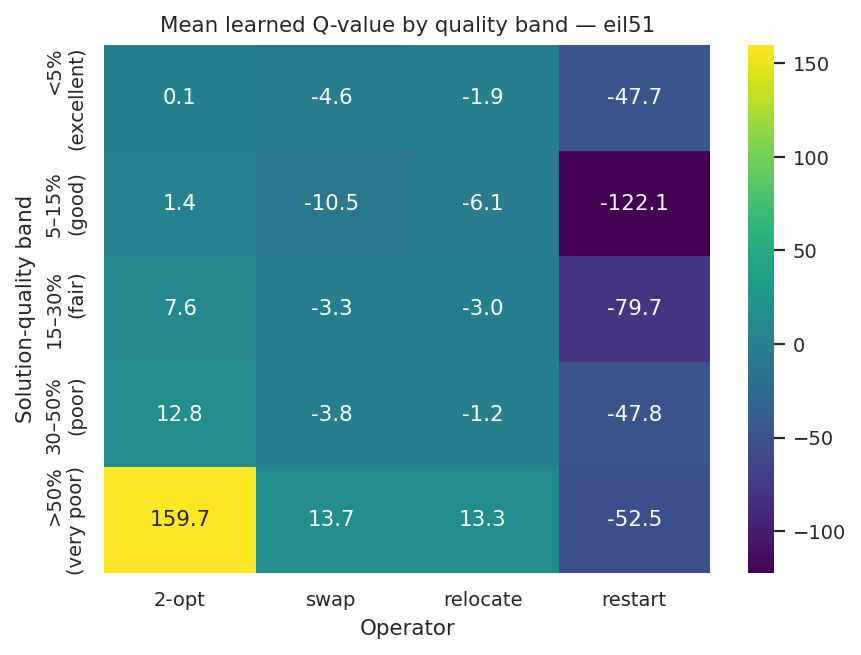
\includegraphics[width=\linewidth]{qtable_eil51.png}\caption{eil51}\end{subfigure}\hfill
\begin{subfigure}{0.49\linewidth}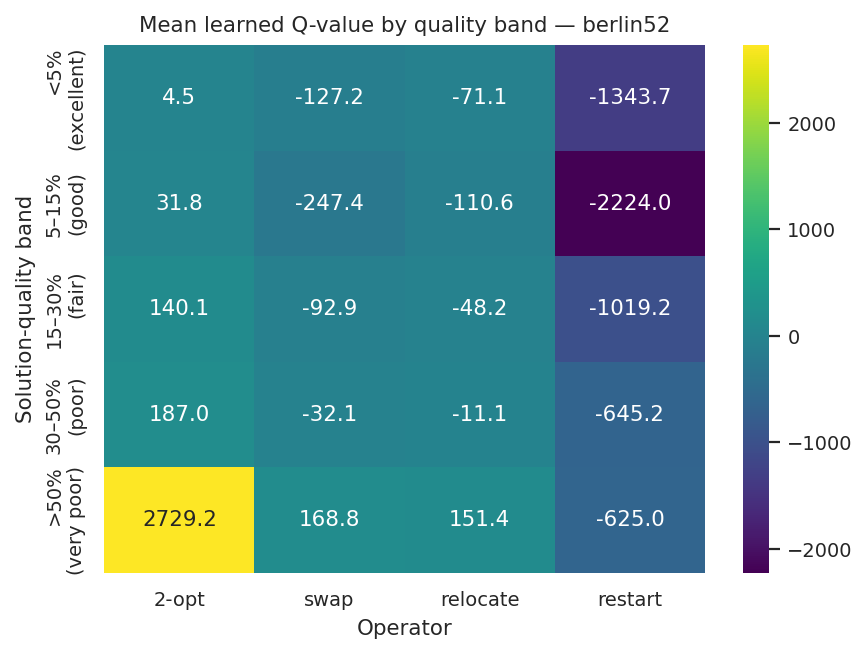
\includegraphics[width=\linewidth]{qtable_berlin52.png}\caption{berlin52}\end{subfigure}
\caption{Average learned Q-values broken down by solution-quality band and
operator. 2-opt commands the highest action-value in most bands; restart
acquires notable value only when solution quality is at its worst.}
\label{fig:qtable}
\end{figure}

\begin{figure}[t]
\centering
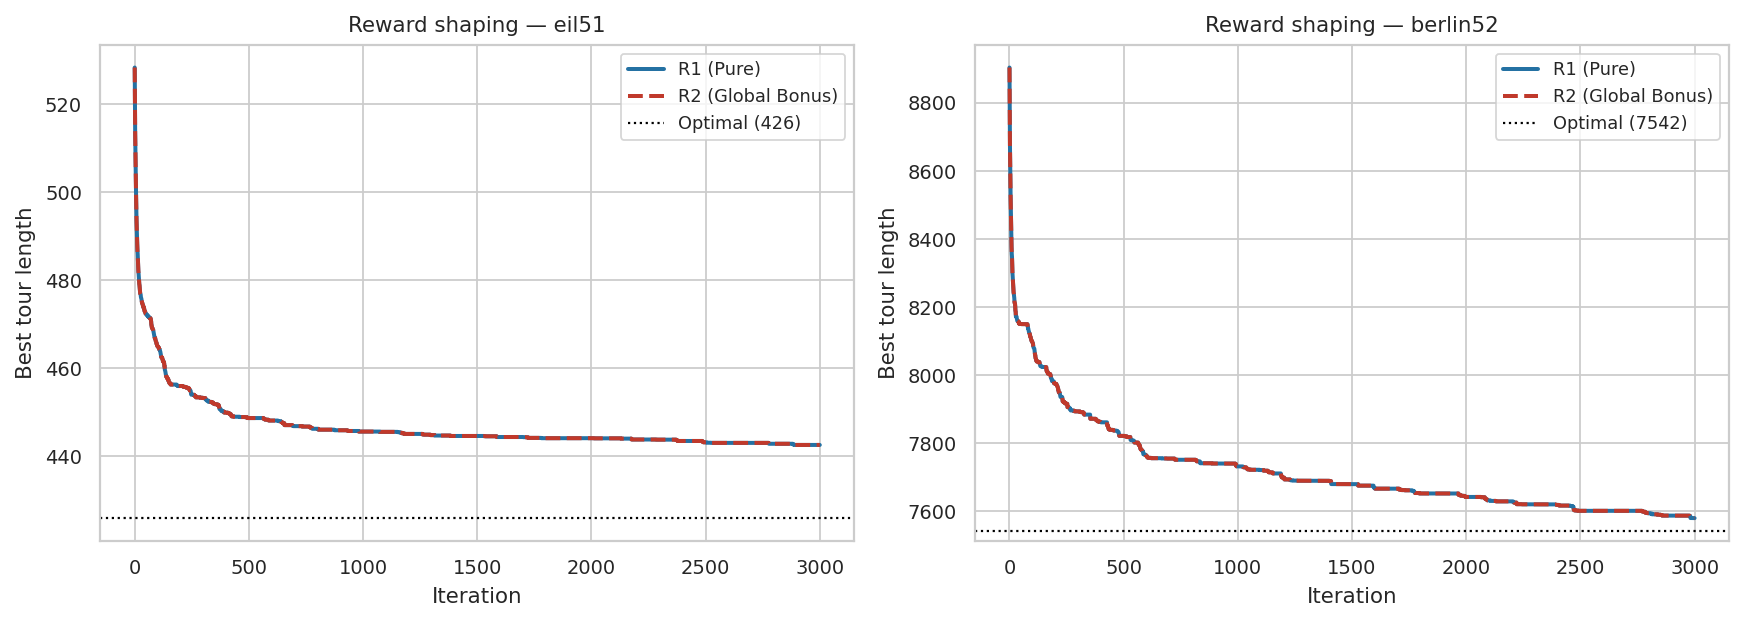
\includegraphics[width=\linewidth]{reward_comparison.png}
\caption{Reward-shaping comparison: $R_1$ (raw improvement) against $R_2$
(raw improvement plus a global-best bonus). Convergence curves overlap
completely on both training instances.}
\label{fig:reward}
\end{figure}

\begin{figure}[t]
\centering
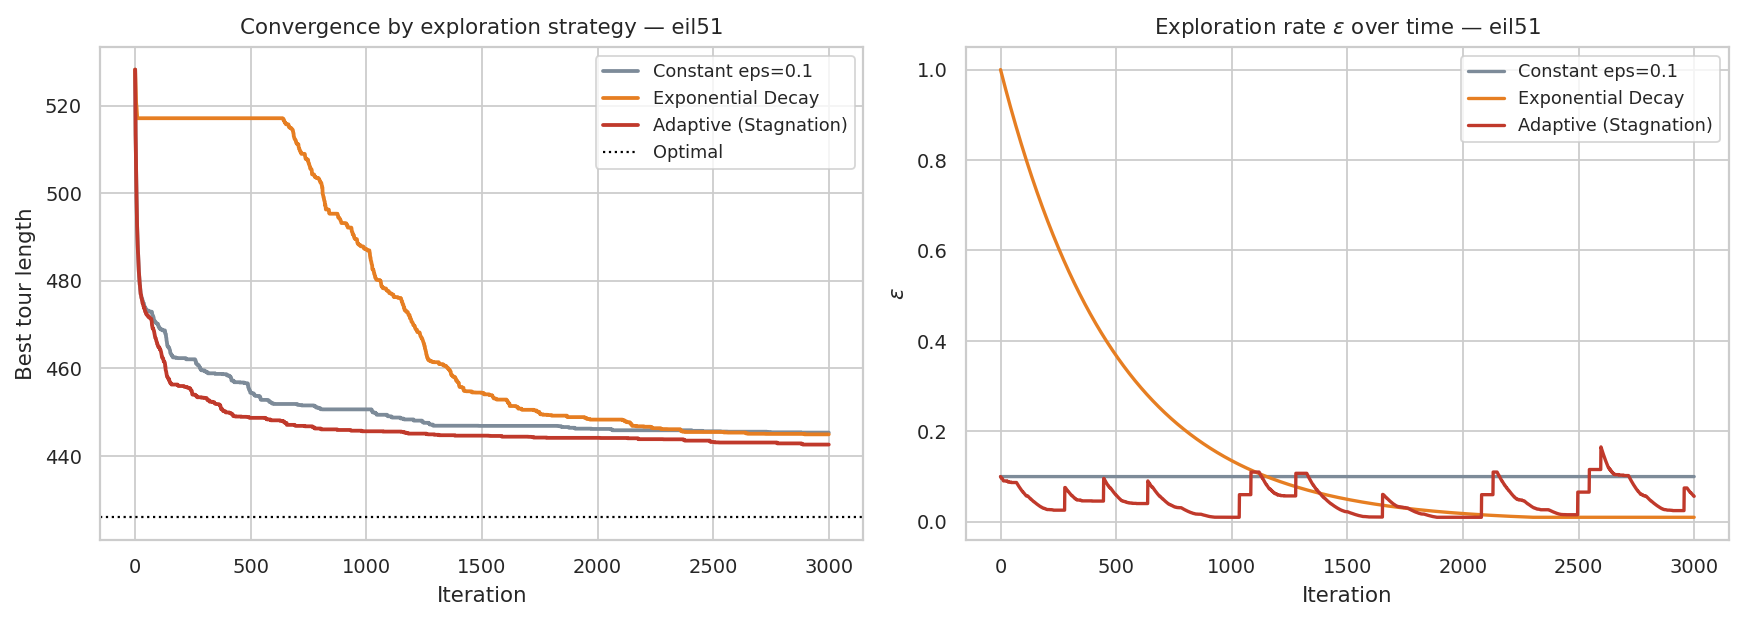
\includegraphics[width=0.82\linewidth]{epsilon_comparison.png}\\[0.2em]
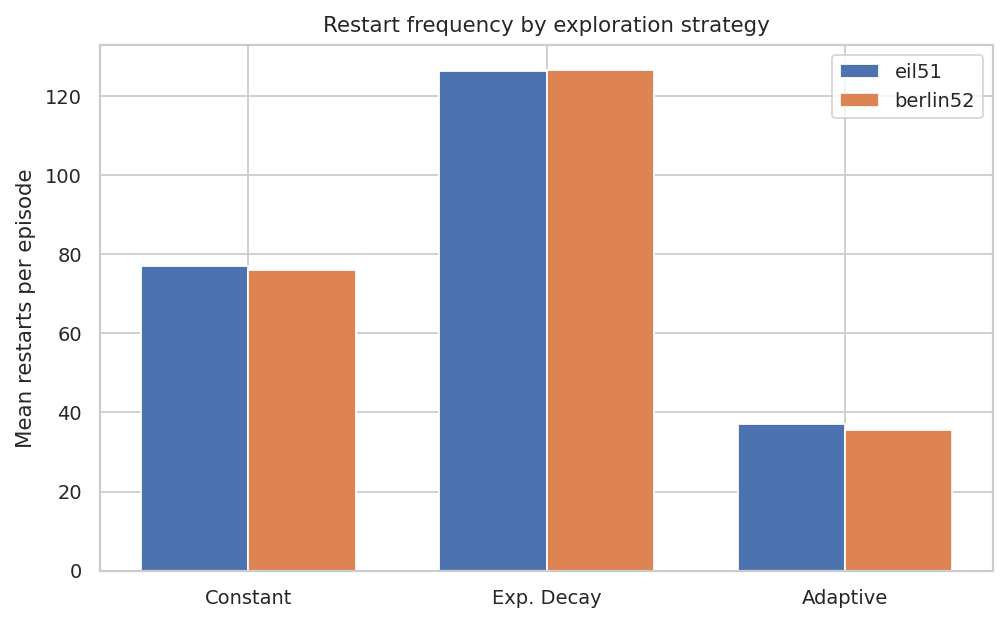
\includegraphics[width=0.44\linewidth]{epsilon_restarts.png}
\caption{Upper panel: convergence and $\varepsilon$ trajectory for each
schedule on eil51. Lower panel: average restarts per episode. The adaptive
schedule achieves the lowest final tour length while invoking the fewest
restarts.}
\label{fig:eps}
\end{figure}

\begin{figure}[t]
\centering
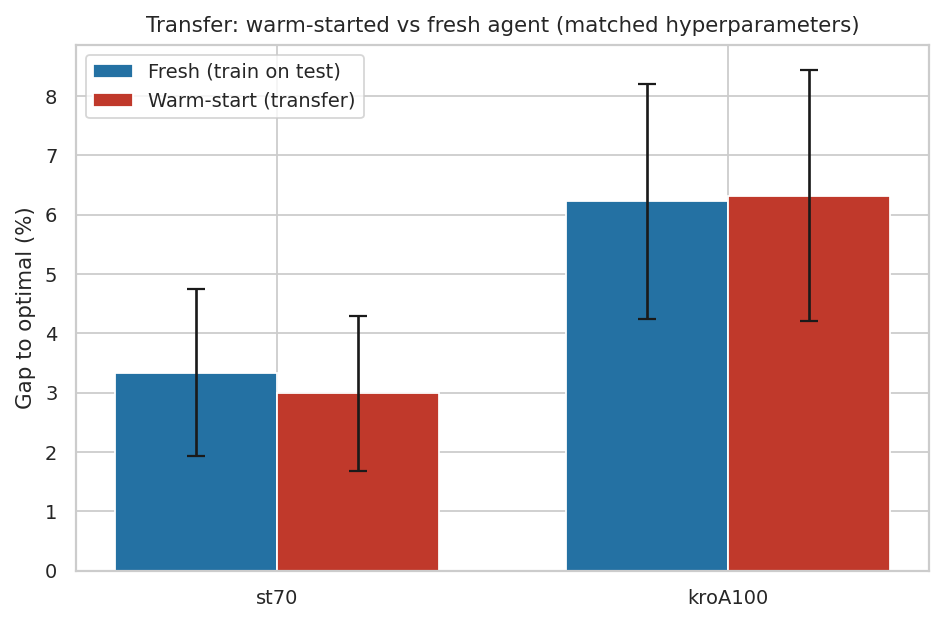
\includegraphics[width=0.65\linewidth]{generalization.png}
\caption{Cross-instance transfer under controlled hyper-parameters. The
difference between a warm-started and a from-scratch agent fails to reach
statistical significance on either held-out instance.}
\label{fig:gen}
\end{figure}

\begin{figure}[t]
\centering
\begin{subfigure}{0.34\linewidth}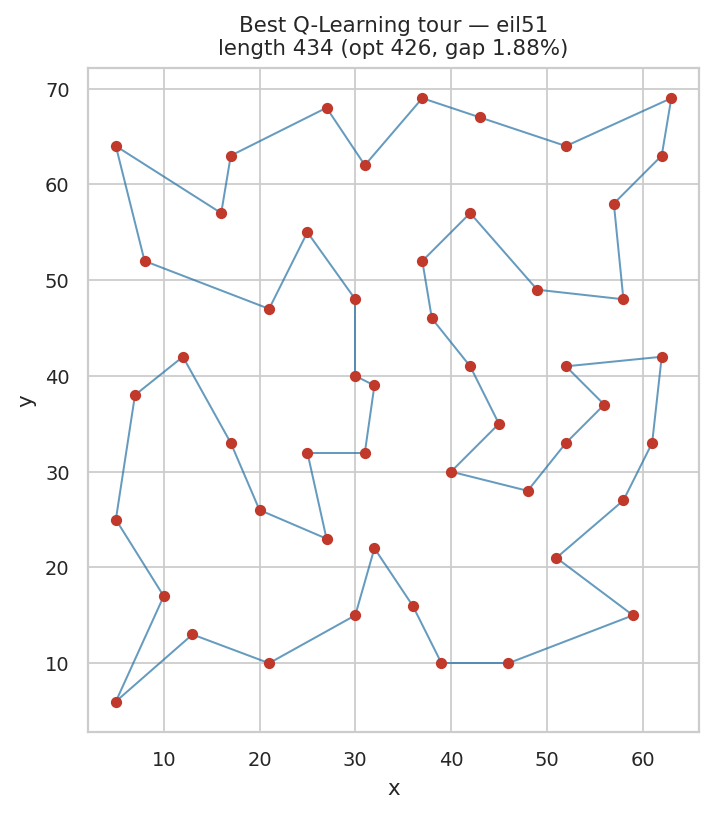
\includegraphics[width=\linewidth]{tour_eil51.png}\caption{eil51}\end{subfigure}\hfill
\begin{subfigure}{0.40\linewidth}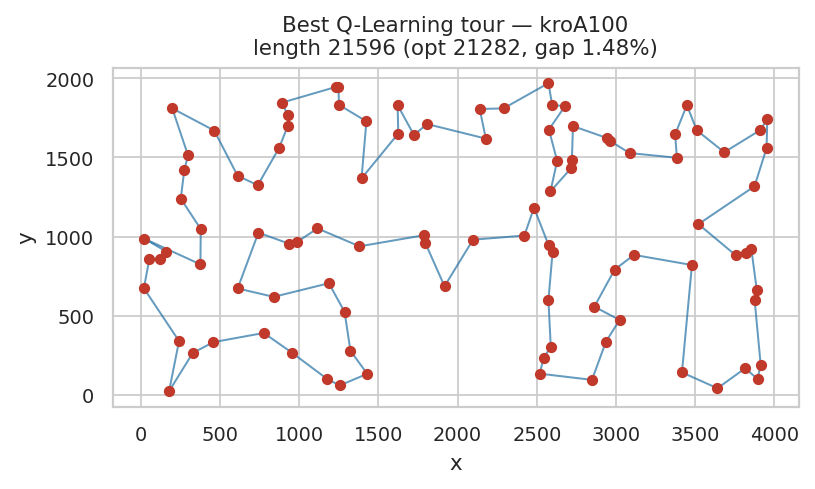
\includegraphics[width=\linewidth]{tour_kroA100.png}\caption{kroA100}\end{subfigure}
\caption{Shortest tours produced by the Q-learning agent on eil51 and kroA100.}
\label{fig:tour}
\end{figure}

% ============================================================
\begin{thebibliography}{99}
\itemsep0.15em
\bibitem{croes1958} G.~A. Croes, ``A method for solving traveling-salesman problems,'' \emph{Operations Research}, vol.~6, no.~6, pp.~791--812, 1958.
\bibitem{lin1973} S.~Lin and B.~W. Kernighan, ``An effective heuristic algorithm for the traveling-salesman problem,'' \emph{Operations Research}, vol.~21, no.~2, pp.~498--516, 1973.
\bibitem{helsgaun2000} K.~Helsgaun, ``An effective implementation of the Lin--Kernighan traveling salesman heuristic,'' \emph{European Journal of Operational Research}, vol.~126, no.~1, pp.~106--130, 2000.
\bibitem{lourenco2003} H.~R. Louren\c{c}o, O.~C. Martin, and T.~St\"utzle, ``Iterated local search,'' in \emph{Handbook of Metaheuristics}, F.~Glover and G.~A. Kochenberger, Eds. Boston: Kluwer, 2003, pp.~320--353.
\bibitem{watkins1992} C.~J.~C.~H. Watkins and P.~Dayan, ``Q-learning,'' \emph{Machine Learning}, vol.~8, no.~3--4, pp.~279--292, 1992.
\bibitem{sutton2018} R.~S. Sutton and A.~G. Barto, \emph{Reinforcement Learning: An Introduction}, 2nd ed. Cambridge, MA: MIT Press, 2018.
\bibitem{tokic2010} M.~Tokic, ``Adaptive $\varepsilon$-greedy exploration in reinforcement learning based on value differences,'' in \emph{KI 2010: Advances in Artificial Intelligence}, LNCS vol.~6359. Berlin: Springer, 2010, pp.~203--210.
\bibitem{burke2013} E.~K. Burke, M.~Gendreau, M.~Hyde, G.~Kendall, G.~Ochoa, E.~\"Ozcan, and R.~Qu, ``Hyper-heuristics: a survey of the state of the art,'' \emph{Journal of the Operational Research Society}, vol.~64, no.~12, pp.~1695--1724, 2013.
\bibitem{meignan2010} D.~Meignan, A.~Koukam, and J.-C. Cr\'eput, ``Coalition-based metaheuristic: a self-adaptive metaheuristic using reinforcement learning and mimetism,'' \emph{Journal of Heuristics}, vol.~16, no.~6, pp.~859--879, 2010.
\bibitem{dacosta2020} P.~da Costa, J.~Rhuggenaath, Y.~Zhang, and A.~Akcay, ``Learning 2-opt heuristics for the traveling salesman problem via deep reinforcement learning,'' in \emph{Proc. 12th Asian Conf. on Machine Learning (ACML)}, PMLR vol.~129, 2020, pp.~465--480.
\bibitem{reinelt1991} G.~Reinelt, ``TSPLIB---a traveling salesman problem library,'' \emph{ORSA Journal on Computing}, vol.~3, no.~4, pp.~376--384, 1991.
\end{thebibliography}

\end{document}
